\hypertarget{gtkexpression}{%
\section{GtkExpression}\label{gtkexpression}}

GtkExpression is a fundamental type. It is not a descendant of GObject.
GtkExpression provides a way to describe references to values.
GtkExpression needs to be evaluated to obtain a value.

It is similar to arithmetic calculation.

\begin{lstlisting}
1 + 2 = 3
\end{lstlisting}

\passthrough{\lstinline!1+2!} is an expression. It shows the way how to
calculate. \passthrough{\lstinline!3!} is the value comes from the
expression. Evaluation is to calculate the expression and get the value.

GtkExpression is a way to get a value. Evaluation is like a calculation.
A value is got by evaluating the expression.

First, I want to show you the C file of the example for GtkExpression.
Its name is \passthrough{\lstinline!exp.c!} and located under
src/expression directory. You don't need to understand the details now,
just look at it. It will be explained in the next subsection.

\begin{lstlisting}[language=C, numbers=left]
#include <gtk/gtk.h>

GtkWidget *win1;
int width, height;
GtkExpressionWatch *watch_width;
GtkExpressionWatch *watch_height;

/* Notify is called when "default-width" or "default-height" property is changed. */
static void
notify (gpointer user_data) {
  GValue value = G_VALUE_INIT;
  char *title;

  if (watch_width && gtk_expression_watch_evaluate (watch_width, &value))
    width = g_value_get_int (&value);
  g_value_unset (&value);
  if (watch_height && gtk_expression_watch_evaluate (watch_height, &value))
    height = g_value_get_int (&value);
  g_value_unset (&value);
  title = g_strdup_printf ("%d x %d", width, height);
  gtk_window_set_title (GTK_WINDOW (win1), title);
  g_free (title);
}

/* This function is used by closure tag in exp.ui. */
char *
set_title (GtkWidget *win, int width, int height) {
  return g_strdup_printf ("%d x %d", width, height);
}

/* ----- activate, open, startup handlers ----- */
static void
app_activate (GApplication *application) {
  GtkApplication *app = GTK_APPLICATION (application);
  GtkWidget *box;
  GtkWidget *label1, *label2, *label3;
  GtkWidget *entry;
  GtkEntryBuffer *buffer;
  GtkBuilder *build;
  GtkExpression *expression, *expression1, *expression2;
  GValue value = G_VALUE_INIT;
  char *s;

  /* Creates GtkApplicationWindow instance. */
  /* The codes below are complecated. It does the same as "win1 = gtk_application_window_new (app);". */
  /* The codes are written just to show how to use GtkExpression. */
  expression = gtk_cclosure_expression_new (GTK_TYPE_APPLICATION_WINDOW, NULL, 0, NULL,
                 G_CALLBACK (gtk_application_window_new), NULL, NULL);
  if (gtk_expression_evaluate (expression, app, &value)) {
    win1 = GTK_WIDGET (g_value_get_object (&value)); /* GtkApplicationWindow */
    g_object_ref (win1);
    g_print ("Got GtkApplicationWindow instance.\n");
  }else
    g_print ("The cclosure expression wasn't evaluated correctly.\n");
  gtk_expression_unref (expression);
  g_value_unset (&value);    /* At the same time, the reference count of win1 is decreased by one. */

  /* Builds a window with components */
  box = gtk_box_new (GTK_ORIENTATION_VERTICAL, 10);
  label1 = gtk_label_new (NULL);
  label2 = gtk_label_new (NULL);
  label3 = gtk_label_new (NULL);
  buffer = gtk_entry_buffer_new (NULL, 0);
  entry = gtk_entry_new_with_buffer (buffer);
  gtk_box_append (GTK_BOX (box), label1);
  gtk_box_append (GTK_BOX (box), label2);
  gtk_box_append (GTK_BOX (box), label3);
  gtk_box_append (GTK_BOX (box), entry);
  gtk_window_set_child (GTK_WINDOW (win1), box);

  /* Constant expression */
  expression = gtk_constant_expression_new (G_TYPE_INT,100);
  if (gtk_expression_evaluate (expression, NULL, &value)) {
    s = g_strdup_printf ("%d", g_value_get_int (&value));
    gtk_label_set_text (GTK_LABEL (label1), s);
    g_free (s);
  } else
    g_print ("The constant expression wasn't evaluated correctly.\n");
  gtk_expression_unref (expression);
  g_value_unset (&value);

  /* Property expression and binding*/
  expression1 = gtk_property_expression_new (GTK_TYPE_ENTRY, NULL, "buffer");
  expression2 = gtk_property_expression_new (GTK_TYPE_ENTRY_BUFFER, expression1, "text");
  gtk_expression_bind (expression2, label2, "label", entry);

  /* Constant expression instead of "this" instance */
  expression1 = gtk_constant_expression_new (GTK_TYPE_APPLICATION, app);
  expression2 = gtk_property_expression_new (GTK_TYPE_APPLICATION, expression1, "application-id");
  if (gtk_expression_evaluate (expression2, NULL, &value))
    gtk_label_set_text (GTK_LABEL (label3), g_value_get_string (&value));
  else
    g_print ("The property expression wasn't evaluated correctly.\n");
  gtk_expression_unref (expression1); /* expression 2 is also freed. */
  g_value_unset (&value);

  width = 800;
  height = 600;
  gtk_window_set_default_size (GTK_WINDOW (win1), width, height);
  notify(NULL);

  /* GtkExpressionWatch */
  expression1 = gtk_property_expression_new (GTK_TYPE_WINDOW, NULL, "default-width");
  watch_width = gtk_expression_watch (expression1, win1, notify, NULL, NULL);
  expression2 = gtk_property_expression_new (GTK_TYPE_WINDOW, NULL, "default-height");
  watch_height = gtk_expression_watch (expression2, win1, notify, NULL, NULL);

  gtk_widget_show (win1);

  /* Builds a window with exp.ui resource */
  build = gtk_builder_new_from_resource ("/com/github/ToshioCP/exp/exp.ui");
  GtkWidget *win2 = GTK_WIDGET (gtk_builder_get_object (build, "win2"));
  gtk_window_set_application (GTK_WINDOW (win2), app);
  g_object_unref (build);

  gtk_widget_show (win2);
}

static void
app_startup (GApplication *application) {
}

#define APPLICATION_ID "com.github.ToshioCP.exp"

int
main (int argc, char **argv) {
  GtkApplication *app;
  int stat;

  app = gtk_application_new (APPLICATION_ID, G_APPLICATION_FLAGS_NONE);

  g_signal_connect (app, "startup", G_CALLBACK (app_startup), NULL);
  g_signal_connect (app, "activate", G_CALLBACK (app_activate), NULL);
/*  g_signal_connect (app, "open", G_CALLBACK (app_open), NULL);*/

  stat =g_application_run (G_APPLICATION (app), argc, argv);
  g_object_unref (app);
  return stat;
}
\end{lstlisting}

\passthrough{\lstinline!exp.c!} consists of five functions.

\begin{itemize}
\tightlist
\item
  \passthrough{\lstinline!notify!}
\item
  \passthrough{\lstinline!set\_title!}
\item
  \passthrough{\lstinline!app\_activate!}. This is a handler of
  ``activate'' signal on GtkApplication instance.
\item
  \passthrough{\lstinline!app\_startup!}. This is a handler of
  ``startup''signal. But nothing is done in this function.
\item
  \passthrough{\lstinline!main!}.
\end{itemize}

The function \passthrough{\lstinline!app\_activate!} is an actual main
body in \passthrough{\lstinline!exp.c!}.

\hypertarget{constant-expression}{%
\subsection{Constant expression}\label{constant-expression}}

Constant expression provides constant value or instance when it is
evaluated.

\begin{itemize}
\tightlist
\item
  72-80: A constant expression. It is extracted and put into here.
\end{itemize}

\begin{lstlisting}[language=C]
  expression = gtk_constant_expression_new (G_TYPE_INT,100);
  if (gtk_expression_evaluate (expression, NULL, &value)) {
    s = g_strdup_printf ("%d", g_value_get_int (&value));
    gtk_label_set_text (GTK_LABEL (label1), s);
    g_free (s);
  } else
    g_print ("The constant expression wasn't evaluated correctly.\n");
  gtk_expression_unref (expression);
  g_value_unset (&value);
\end{lstlisting}

\begin{itemize}
\tightlist
\item
  Constant expression is created with
  \passthrough{\lstinline!gtk\_constant\_expression\_new!} function. The
  parameter of the function is a type (GType) and a value (or instance).
\item
  \passthrough{\lstinline!gtk\_expression\_evaluate!} evaluates the
  expression. It has three parameters, the expression to evaluate,
  \passthrough{\lstinline!this!} instance and GValue for being set with
  the value. \passthrough{\lstinline!this!} instance isn't necessary for
  constant expressions. Therefore the second argument is NULL.
  \passthrough{\lstinline!gtk\_expression\_evaluate!} returns TRUE if it
  successfully evaluates the expression. Otherwise it returns FALSE.
\item
  If it returns TRUE, the GValue \passthrough{\lstinline!value!} is set
  with the value of the expression. The type of the value is int.
  \passthrough{\lstinline!g\_strdup\_printf!} converts the value to a
  string \passthrough{\lstinline!s!}.
\item
  GtkLabel \passthrough{\lstinline!label1!} is set with
  \passthrough{\lstinline!s!}. The string \passthrough{\lstinline!s!}
  needs to be freed.
\item
  If the evaluation fails a message is outputted to stderr.
\item
  The expression and GValue are freed.
\end{itemize}

Constant expression is usually used to give a constant value or instance
to another expression.

\hypertarget{property-expression}{%
\subsection{Property expression}\label{property-expression}}

Property expression looks up a property in a GObject object. For
example, a property expression that refers ``label'' property in
GtkLabel object is created like this.

\begin{lstlisting}[language=C]
expression = gtk_property_expression_new (GTK_TYPE_LABEL, another_expression, "label");
\end{lstlisting}

\passthrough{\lstinline!another\_expression!} is expected to give a
GtkLabel instance when it is evaluated. For example,

\begin{lstlisting}[language=C]
label = gtk_label_new ("Hello");
another_expression = gtk_constant_expression_new (GTK_TYPE_LABEL, label);
expression = gtk_property_expression_new (GTK_TYPE_LABEL, another_expression, "label");
\end{lstlisting}

If \passthrough{\lstinline!expression!} is evaluated, the second
parameter \passthrough{\lstinline!another\_expression!} is evaluated in
advance. The value of \passthrough{\lstinline!another\_expression!} is
\passthrough{\lstinline!label!} (GtkLabel instance). Then,
\passthrough{\lstinline!expression!} looks up ``label'' property of
\passthrough{\lstinline!label!} and the evaluation result is ``Hello''.

In the example above, the second argument of
\passthrough{\lstinline!gtk\_property\_expression\_new!} is another
expression. But the second argument can be NULL. If it is NULL,
\passthrough{\lstinline!this!} instance is used instead.
\passthrough{\lstinline!this!} is given by
\passthrough{\lstinline!gtk\_expression\_evaluate!} function at the
evaluation.

Now look at \passthrough{\lstinline!exp.c!}. The lines from 83 to 85 is
extracted here.

\begin{lstlisting}[language=C]
  expression1 = gtk_property_expression_new (GTK_TYPE_ENTRY, NULL, "buffer");
  expression2 = gtk_property_expression_new (GTK_TYPE_ENTRY_BUFFER, expression1, "text");
  gtk_expression_bind (expression2, label2, "label", entry);
\end{lstlisting}

\begin{itemize}
\tightlist
\item
  \passthrough{\lstinline!expression1!} looks up ``buffer'' property of
  \passthrough{\lstinline!this!} object, which is
  \passthrough{\lstinline!GTK\_TYPE\_ENTRY!} type.
\item
  \passthrough{\lstinline!expression2!} looks up ``text'' property of
  GtkEntryBuffer object given by \passthrough{\lstinline!epression1!}.
\item
  \passthrough{\lstinline!gtk\_expression\_bind!} binds a property to a
  value given by the expression. In this program, it binds a ``label''
  property in \passthrough{\lstinline!label2!} to the value evaluated
  with \passthrough{\lstinline!expresion2!} with
  \passthrough{\lstinline!entry!} as \passthrough{\lstinline!this!}
  object. The evaluation process is as follows.

  \begin{enumerate}
  \def\labelenumi{\arabic{enumi}.}
  \tightlist
  \item
    \passthrough{\lstinline!expression2!} is evaluated. But it includes
    \passthrough{\lstinline!expression1!} so
    \passthrough{\lstinline!expression1!} is evaluated in advance.
  \item
    Because the second argument of \passthrough{\lstinline!expression1!}
    is NULL, \passthrough{\lstinline!this!} object is used.
    \passthrough{\lstinline!this!} is given by
    \passthrough{\lstinline!gtk\_expression\_bind!}. It is
    \passthrough{\lstinline!entry!} (GtkEntry instance).
    \passthrough{\lstinline!expression1!} looks up ``buffer'' property
    in \passthrough{\lstinline!entry!}. It is a GtkEntryBuffer instance
    \passthrough{\lstinline!buffer!}. (See line 64 in
    \passthrough{\lstinline!exp.c!}.)
  \item
    Then, \passthrough{\lstinline!expression2!} looks up ``text''
    property in \passthrough{\lstinline!buffer!}. It is a text held in
    \passthrough{\lstinline!entry!}.
  \item
    The text is assigned to ``label'' property in
    \passthrough{\lstinline!label2!}.
  \end{enumerate}
\item
  \passthrough{\lstinline!gtk\_expression\_bind!} creates a
  GtkExpressionWatch. (But it isn't assigned to a variable in the
  program above. If you want to keep the GtkExpressionWatch instance,
  assign it to a variable.)
\end{itemize}

\begin{lstlisting}[language=C]
  GtkExpressionWatch *watch;
  watch = gtk_expression_bind (expression2, label2, "label", entry);
\end{lstlisting}

\begin{itemize}
\tightlist
\item
  Whenever the value from \passthrough{\lstinline!expression2!} changes,
  it evaluates \passthrough{\lstinline!expression2!} and set ``label''
  property in \passthrough{\lstinline!label2!}. So, the change of the
  text in \passthrough{\lstinline!entry!} makes the ``label'' property
  reflect it immediately.
\end{itemize}

\hypertarget{closure-expression}{%
\subsection{Closure expression}\label{closure-expression}}

Closure expression calls closure when it is evaluated. A closure is a
generic representation of a callback (a pointer to a function). For
information about closure, see
\href{https://docs.gtk.org/gobject/concepts.html\#the-gobject-messaging-system}{GObject
API Reference, The GObject messaging system}. A closure expression is
created with \passthrough{\lstinline!gtk\_cclosure\_expression\_new!}
function.

\begin{lstlisting}[language=C]
GtkExpression *
gtk_cclosure_expression_new (GType value_type,
                             GClosureMarshal marshal,
                             guint n_params,
                             GtkExpression **params,
                             GCallback callback_func,
                             gpointer user_data,
                             GClosureNotify user_destroy);
\end{lstlisting}

\begin{itemize}
\tightlist
\item
  \passthrough{\lstinline!value\_type!} is the type of the value when it
  is evaluated.
\item
  \passthrough{\lstinline!marshal!} is a marshaller. You can assign
  NULL. If it is NULL, then
  \passthrough{\lstinline!g\_cclosure\_marshal\_generic ()!} is used as
  a marshaller. It is a generic marshaller function implemented via
  libffi.
\item
  \passthrough{\lstinline!n\_params!} is the number of parameters.
\item
  \passthrough{\lstinline!params!} points expressions for each parameter
  of the call back function.
\item
  \passthrough{\lstinline!callback\_func!} is a callback function.
\item
  \passthrough{\lstinline!user\_data!} is user data. You can add it for
  the closure. It is like \passthrough{\lstinline!user\_data!} in
  \passthrough{\lstinline!g\_signal\_connect!}. If it is not necessary,
  assign NULL.
\item
  \passthrough{\lstinline!user\_destroy!} is a destroy notify for
  \passthrough{\lstinline!user\_data!}. It is called to destroy
  \passthrough{\lstinline!user\_data!} when it is no longer needed. If
  NULL is assigned to \passthrough{\lstinline!user\_data!}, assign NULL
  to \passthrough{\lstinline!user\_destroy!}, too.
\end{itemize}

The following is extracted from \passthrough{\lstinline!exp.c!}. It is
from line 47 to line 56.

\begin{lstlisting}[language=C]
expression = gtk_cclosure_expression_new (GTK_TYPE_APPLICATION_WINDOW, NULL, 0, NULL,
               G_CALLBACK (gtk_application_window_new), NULL, NULL);
if (gtk_expression_evaluate (expression, app, &value)) {
  win1 = GTK_WIDGET (g_value_get_object (&value)); /* GtkApplicationWindow */
  g_object_ref (win1);
  g_print ("Got GtkApplicationWindow object.\n");
}else
  g_print ("The cclosure expression wasn't evaluated correctly.\n");
gtk_expression_unref (expression);
g_value_unset (&value);    /* At the same time, the reference count of win1 is decreased by one. */
\end{lstlisting}

The callback function is
\passthrough{\lstinline!gtk\_application\_window\_new!}. This function
has one parameter which is an instance of GtkApplication. And it returns
newly created GtkApplicationWindow instance. So, the first argument is
\passthrough{\lstinline!GTK\_TYPE\_APPLICATION\_WINDOW!} which is the
type of the return value. The second argument is NULL so general
marshaller \passthrough{\lstinline!g\_cclosure\_marshal\_generic ()!}
will be used. I think assigning NULL works in most cases when you
program in C language.

The arguments given to the call back function are
\passthrough{\lstinline!this!} object and parameters which are the
fourth argument of
\passthrough{\lstinline!gtk\_cclosure\_expression\_new!}. So, the number
of arguments is \passthrough{\lstinline!n\_params + 1!}. Because
\passthrough{\lstinline!gtk\_application\_window\_new!} has one
parameter, so \passthrough{\lstinline!n\_params!} is zero and
\passthrough{\lstinline!**params!} is NULL. No user data is necessary,
so \passthrough{\lstinline!user\_data!} and
\passthrough{\lstinline!user\_destroy!} are NULL.

\passthrough{\lstinline!gtk\_expression\_evaluate!} evaluates the
expression. \passthrough{\lstinline!this!} instance will be the first
argument for \passthrough{\lstinline!gtk\_application\_window\_new!}, so
it is \passthrough{\lstinline!app!}.

If the evaluation succeeds, the GValue \passthrough{\lstinline!value!}
holds a newly created GtkApplicationWindow instance. It is assigned to
\passthrough{\lstinline!win1!}. The GValue will be unset when it is no
longer used. And when it is unset, the GtkApplicationWindow instance
will be released and its reference count will be decreased by one. It is
necessary to increase the reference count by one in advance to keep the
instance. \passthrough{\lstinline!gtk\_expression\_unref!} frees
\passthrough{\lstinline!expression!} and \passthrough{\lstinline!value!}
is unset.

As a result, we got a GtkApplicationWindow instance
\passthrough{\lstinline!win1!}. We can do the same by:

\begin{lstlisting}[language=C]
win1 = gtk_application_window_new (app);
\end{lstlisting}

The example is more complicated and not practical than this one line
code. The aim of the example is just to show how closure expression
works.

Closure expression is flexible than other type of expression because you
can specify your own callback function.

\hypertarget{gtkexpressionwatch}{%
\subsection{GtkExpressionWatch}\label{gtkexpressionwatch}}

GtkExpressionWatch watches an expression and if the value of the
expression changes it calls its notify handler.

The example uses GtkExpressionWatch in the line 103 to 106.

\begin{lstlisting}[language=C]
expression1 = gtk_property_expression_new (GTK_TYPE_WINDOW, NULL, "default-width");
watch_width = gtk_expression_watch (expression1, win1, notify, NULL, NULL);
expression2 = gtk_property_expression_new (GTK_TYPE_WINDOW, NULL, "default-height");
watch_height = gtk_expression_watch (expression2, win1, notify, NULL, NULL);
\end{lstlisting}

The expressions above refer to ``default-width'' and ``default-height''
properties of GtkWindow. The variable
\passthrough{\lstinline!watch\_width!} watches
\passthrough{\lstinline!expression1!}. The second argument
\passthrough{\lstinline!win1!} is \passthrough{\lstinline!this!}
instance for \passthrough{\lstinline!expression1!}. So,
\passthrough{\lstinline!watch\_width!} watches the value of
``default-width'' property of \passthrough{\lstinline!win1!}. If the
value changes, it calls \passthrough{\lstinline!notify!} handler. The
fourth and fifth arguments are NULL because no user data is necessary.

The variable \passthrough{\lstinline!watch\_height!} connects
\passthrough{\lstinline!notify!} handler to
\passthrough{\lstinline!expression2!}. So,
\passthrough{\lstinline!notiry!} is also called when ``default-height''
changes.

The handler \passthrough{\lstinline!norify!} is as follows.

\begin{lstlisting}[language=C, numbers=left]
static void
notify (gpointer user_data) {
  GValue value = G_VALUE_INIT;
  char *title;

  if (watch_width && gtk_expression_watch_evaluate (watch_width, &value))
    width = g_value_get_int (&value);
  g_value_unset (&value);
  if (watch_height && gtk_expression_watch_evaluate (watch_height, &value))
    height = g_value_get_int (&value);
  g_value_unset (&value);
  title = g_strdup_printf ("%d x %d", width, height);
  gtk_window_set_title (GTK_WINDOW (win1), title);
  g_free (title);
}
\end{lstlisting}

\begin{itemize}
\tightlist
\item
  6-11: Evaluates \passthrough{\lstinline!expression1!} and
  \passthrough{\lstinline!expression2!} with
  \passthrough{\lstinline!expression\_watch\_evaluate!} function.
\item
  12: Creates a string \passthrough{\lstinline!title!}. It contains the
  width and height, for example, ``800 x 600''.
\item
  13: Sets the title of \passthrough{\lstinline!win1!} with the string
  \passthrough{\lstinline!title!}.
\end{itemize}

The title of the window reflects the size of the window.

\hypertarget{exp.ui}{%
\subsection{exp.ui}\label{exp.ui}}

\passthrough{\lstinline!exp.c!} builds a GtkWindow instance
\passthrough{\lstinline!win2!} with \passthrough{\lstinline!exp.ui!}.
The ui file \passthrough{\lstinline!exp.ui!} includes tags to create
GtkExpressions. The tags are:

\begin{itemize}
\tightlist
\item
  constant tag to create constant expression
\item
  lookup tag to create property expression
\item
  closure tag to create closure expression
\item
  binding tag to bind a property to an expression
\end{itemize}

The window \passthrough{\lstinline!win2!} behaves like
\passthrough{\lstinline!win1!}. Because similar expressions are built
with the ui file.

\begin{lstlisting}[language=XML, numbers=left]
<?xml version="1.0" encoding="UTF-8"?>
<interface>
  <object class="GtkWindow" id="win2">
    <binding name="title">
      <closure type="gchararray" function="set_title">
        <lookup name="default-width" type="GtkWindow"></lookup>
        <lookup name="default-height" type="GtkWindow"></lookup>
      </closure>
    </binding>
    <property name="default-width">600</property>
    <property name="default-height">400</property>
    <child>
      <object class="GtkBox">
        <property name="orientation">GTK_ORIENTATION_VERTICAL</property>
        <child>
          <object class="GtkLabel">
            <binding name="label">
              <constant type="gint">100</constant>
            </binding>
          </object>
        </child>
        <child>
          <object class="GtkLabel">
            <binding name="label">
              <lookup name="text">
                <lookup name="buffer">
                  entry
                </lookup>
              </lookup>
            </binding>
          </object>
        </child>
        <child>
          <object class="GtkLabel">
            <binding name="label">
              <lookup name="application-id">
                <lookup name="application">win2</lookup>
              </lookup>
            </binding>
          </object>
        </child>
        <child>
          <object class="GtkEntry" id="entry">
            <property name="buffer">
              <object class="GtkEntryBuffer"></object>
            </property>
          </object>
        </child>
      </object>
    </child>
  </object>
</interface>
\end{lstlisting}

\hypertarget{constant-tag}{%
\subsubsection{Constant tag}\label{constant-tag}}

A constant tag corresponds to a constant expression.

\begin{itemize}
\tightlist
\item
  18: Constant tag. The constant expression is created with the tag. It
  returns 100, the type is ``gint'', when it is evaluated. The type
  ``gint'' is a name of \passthrough{\lstinline!G\_TYPE\_INT!} type.
  Similarly, the types which is registered to the type system has type
  and name. For example, ``gchararray'' is a name of
  \passthrough{\lstinline!G\_TYPE\_STRING!} type. You need to use the
  name of types for the \passthrough{\lstinline!type!}attribute. See
  \href{https://github.com/ToshioCP/Gobject-tutorial/blob/main/gfm/sec5.md\#gvalue}{GObject
  tutorial}.
\item
  17-19: Binding tag corresponds to
  \passthrough{\lstinline!gtk\_expression\_bind!} function.
  \passthrough{\lstinline!name!} attribute specifies the ``label''
  property of the GtkLabel object just before the binding tag. The
  expression returns a int type GValue. On the other hand ``label''
  property holds a string type GValue. When a GValue is copied to
  another GValue, the type is automatically converted if possible. In
  this case, an int \passthrough{\lstinline!100!} is converted to a
  string \passthrough{\lstinline!"100"!}.
\end{itemize}

These binding and constant tag works. But they are not good. A property
tag is more straightforward.

\begin{lstlisting}[language=XML]
<object class="GtkLabel">
  <property name="label">100</property>
</object>
\end{lstlisting}

This example just shows the way how to use constant tag. Constant tag is
mainly used to give a constant argument to a closure.

\hypertarget{lookup-tag}{%
\subsubsection{Lookup tag}\label{lookup-tag}}

A lookup tag corresponds to a property expression. Line 23 to 31 is
copied here.

\begin{lstlisting}[language=XML]
          <object class="GtkLabel">
            <binding name="label">
              <lookup name="text">
                <lookup name="buffer">
                  entry
                </lookup>
              </lookup>
            </binding>
          </object>
\end{lstlisting}

\begin{itemize}
\tightlist
\item
  binding tag binds a ``label'' property in GtkLabel to an expression.
  The expression is defined with a lookup tag.
\item
  The lookup tag defines a property expression looks up a ``text''
  property in the instance which is defined in the next expression. The
  next expression is created with the lookup tag. The expression looks
  up the \passthrough{\lstinline!buffer!} property of the
  \passthrough{\lstinline!entry!} instance. The
  \passthrough{\lstinline!entry!} instance is defined in the line 43. It
  is a GtkEntry \passthrough{\lstinline!entry!}. A lookup tag takes an
  instance in some ways to look up for a property.

  \begin{itemize}
  \tightlist
  \item
    If it has no contents, it takes \passthrough{\lstinline!this!}
    instance when it is evaluated.
  \item
    If it has a content of a tag for an expression, which is constant,
    lookup or closure tag, the value of the expression will be the
    instance to look up when it is evaluated.
  \item
    If it has a content of an id of an object, then the instance of the
    object will be taken as the instance to lookup.
  \end{itemize}
\end{itemize}

As a result, the label of the GtkLabel instance are bound to the text in
the field of GtkEntry. If a user input a text in the field in the
GtkEntry, GtkLabel displays the same text.

Another lookup tag is in the lines from 34 to 40.

\begin{lstlisting}[language=XML]
          <object class="GtkLabel">
            <binding name="label">
              <lookup name="application-id">
                <lookup name="application">win2</lookup>
              </lookup>
            </binding>
          </object>
\end{lstlisting}

\begin{itemize}
\tightlist
\item
  Two expressions are nested.
\item
  A lookup tag looks up ``application-id'' property of the next
  expression.
\item
  The next lookup tag looks up ``application'' property of
  \passthrough{\lstinline!win2!} instance.
\end{itemize}

As a result, the ``label'' property in the GtkLabel instance is bound to
the ``application-id'' property. The nested tag makes a chain like:

\begin{lstlisting}
"label" <= "application-id" <= "application" <= `win2`
\end{lstlisting}

By the way, the application of \passthrough{\lstinline!win2!} is set
after the objects in ui file are built. Look at
\passthrough{\lstinline!exp.c!}.
\passthrough{\lstinline!gtk\_window\_set\_application!} is called after
\passthrough{\lstinline!gtk\_build\_new\_from\_resource!}.

\begin{lstlisting}[language=C]
build = gtk_builder_new_from_resource ("/com/github/ToshioCP/exp/exp.ui");
GtkWidget *win2 = GTK_WIDGET (gtk_builder_get_object (build, "win2"));
gtk_window_set_application (GTK_WINDOW (win2), app);
\end{lstlisting}

Therefore, before the call for
\passthrough{\lstinline!gtk\_window\_set\_application!}, the
``application'' property of \passthrough{\lstinline!win2!} is \emph{not}
set. So, the evaluation of
\passthrough{\lstinline!<lookup name="application">win2</lookup>!}
fails. And the evaluation of
\passthrough{\lstinline!<lookup name="application-id">!} also fails. A
function \passthrough{\lstinline!gtk\_expression\_bind ()!}, which
corresponds to \passthrough{\lstinline!binding!} tag, doesn't update the
target property if the expression fails. So, the ``label'' property
isn't updated at the first evaluation.

Note that an evaluation can fail. The care is especially necessary when
you write a callback for a closure tag which has contents of expressions
like lookup tags. The expressions are given to the callback as an
argument. If an expression fails the argument will be NULL. You need to
check if the argument exactly points the instance that is expected by
the callback.

\hypertarget{closure-tag}{%
\subsubsection{Closure tag}\label{closure-tag}}

The lines from 3 to 9 include a closure tag.

\begin{lstlisting}[language=XML]
  <object class="GtkWindow" id="win2">
    <binding name="title">
      <closure type="gchararray" function="set_title">
        <lookup name="default-width" type="GtkWindow"></lookup>
        <lookup name="default-height" type="GtkWindow"></lookup>
      </closure>
    </binding>
\end{lstlisting}

\begin{itemize}
\tightlist
\item
  A binding tag corresponds to a
  \passthrough{\lstinline!gtk\_expression\_bind!} function.
  \passthrough{\lstinline!name!} attribute specifies the ``title''
  property of \passthrough{\lstinline!win2!}. Binding tag gives
  \passthrough{\lstinline!win2!} as the \passthrough{\lstinline!this!}
  instance to the expressions, which are the contents of the binding
  tag. So, closure tag and lookup tags use
  \passthrough{\lstinline!win2!} as the \passthrough{\lstinline!this!}
  object when they are evaluated.
\item
  A closure tag corresponds to a closure expression. Its callback
  function is \passthrough{\lstinline!set\_title!} and it returns
  ``gchararray'' type, which is ``an array of characters'' i.e.~a
  string. The contents of the closure tag are assigned to parameters of
  the function. So, \passthrough{\lstinline!set\_title!} has three
  parameters, \passthrough{\lstinline!win2!}
  (\passthrough{\lstinline!this!} instance), default width and default
  height.
\item
  Lookup tags correspond to property expressions. They lookup
  ``default-width'' and ``default-height'' properties of
  \passthrough{\lstinline!win2!} (\passthrough{\lstinline!this!}
  instance).
\item
  Binding tab creates GtkExpressionWatch automatically, so ``title''
  property reflects the changes of ``default-width'' and
  ``default-height'' properties.
\end{itemize}

\passthrough{\lstinline!set\_title!} function in
\passthrough{\lstinline!exp.c!} is as follows.

\begin{lstlisting}[language=C, numbers=left]
char *
set_title (GtkWidget *win, int width, int height) {
  return g_strdup_printf ("%d x %d", width, height);
}
\end{lstlisting}

It just creates a string, for example, ``800 x 600'', and returns it.

You've probably been noticed that ui file is easier and clearer than the
corresponding C program. One of the most useful case of GtkExpression is
building GtkListItem instance with GtkBuilderListItemFatory. Such case
has already been described in the prior two sections.

It will be used in the next section to build GtkListItem in
GtkColumnView, which is the most useful view object for GListModel.

\hypertarget{compilation-and-execution}{%
\subsection{Compilation and execution}\label{compilation-and-execution}}

All the sources are in src/expression directory. Change your current
directory to the directory and run meson and ninja. Then, execute the
application.

\begin{lstlisting}
$ meson _build
$ ninja -C _build
$ build/exp
\end{lstlisting}

Then, two windows appear.

\begin{figure}
\centering
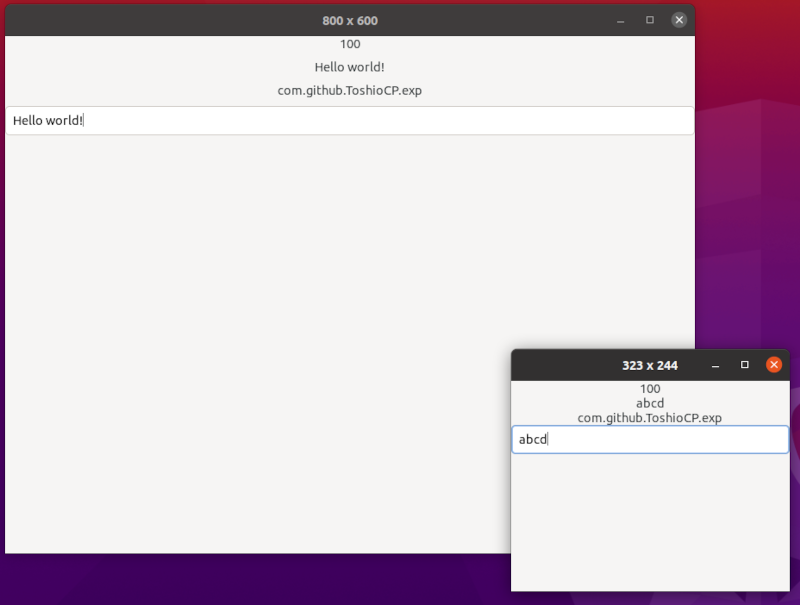
\includegraphics[width=12cm,height=9.1cm]{../image/expression.png}
\caption{Expression}
\end{figure}

If you put some text in the field of the entry, then the same text
appears in the second GtkLabel. Because the ``label'' property of the
second GtkLabel instance is bound to the text in the GtkEntryBuffer.

If you resize the window, then the size appears in the title bar because
the ``title'' property is bound to ``default-width'' and
``default-height'' properties.
